% filename: absorption_refrigerator.tex
\documentclass[tikz]{standalone}
\usepackage{tikz}
\usetikzlibrary{patterns}

\begin{document}
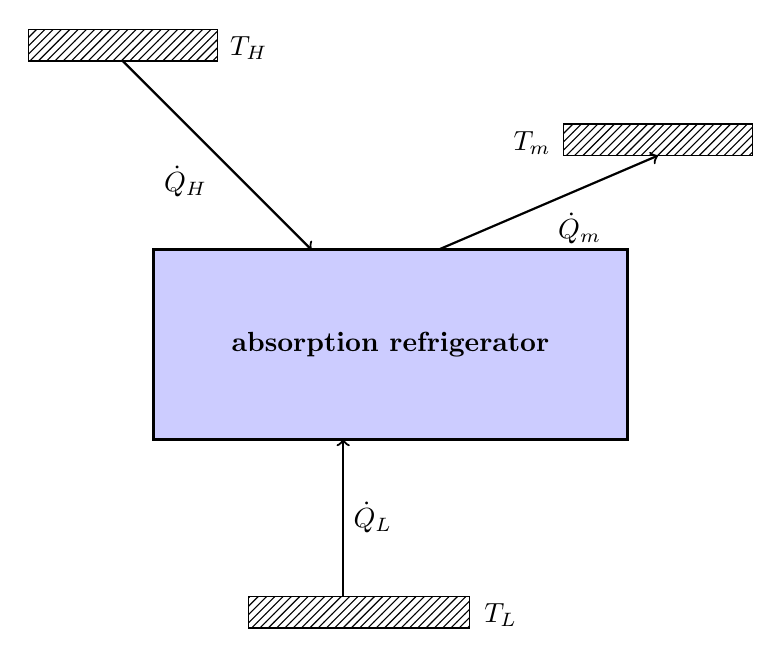
\begin{tikzpicture}[scale=0.8]
    \draw [->, thick]  (5.5, 9.7) -- (8.5, 6.7) node[midway, below left] {$\dot{Q}_{H}$};
    \draw [->, thick]  (10.5, 6.7) -- (14.0, 8.2) node[midway, below right] {$\dot{Q}_{m}$};
    \draw [->, thick]  (9.0, 1.2) -- (9.0, 3.7) node[midway, right] {$\dot{Q}_{L}$};
    \draw[line width=0.5mm] (6.0, 6.7) rectangle (13.5, 3.7);
    \draw[fill=blue!20, draw=black] (6.0, 6.7) rectangle (13.5, 3.7);
    \node at (9.75, 5.2) {\bfseries absorption refrigerator};
    \draw [pattern={north east lines}] (4.0, 10.2) rectangle (7.0, 9.7);
    \node at (7.5, 9.9) {$T_H$};
    \draw [pattern={north east lines}] (12.5, 8.7) rectangle (15.5, 8.2);
    \node at (12.0, 8.4) {$T_m$};
    \draw [pattern={north east lines}] (7.5, 1.2) rectangle (11.0, 0.7);
    \node at (11.5, 0.9) {$T_L$};
\end{tikzpicture}
\end{document}
